% Options for packages loaded elsewhere
\PassOptionsToPackage{unicode}{hyperref}
\PassOptionsToPackage{hyphens}{url}
%
\documentclass[
  12 pt,
  a4paper,
]{article}
\usepackage{amsmath,amssymb}
\usepackage{setspace}
\usepackage{iftex}
\ifPDFTeX
  \usepackage[T1]{fontenc}
  \usepackage[utf8]{inputenc}
  \usepackage{textcomp} % provide euro and other symbols
\else % if luatex or xetex
  \usepackage{unicode-math} % this also loads fontspec
  \defaultfontfeatures{Scale=MatchLowercase}
  \defaultfontfeatures[\rmfamily]{Ligatures=TeX,Scale=1}
\fi
\usepackage{lmodern}
\ifPDFTeX\else
  % xetex/luatex font selection
  \setmainfont[]{Times New Roman}
\fi
% Use upquote if available, for straight quotes in verbatim environments
\IfFileExists{upquote.sty}{\usepackage{upquote}}{}
\IfFileExists{microtype.sty}{% use microtype if available
  \usepackage[]{microtype}
  \UseMicrotypeSet[protrusion]{basicmath} % disable protrusion for tt fonts
}{}
\makeatletter
\@ifundefined{KOMAClassName}{% if non-KOMA class
  \IfFileExists{parskip.sty}{%
    \usepackage{parskip}
  }{% else
    \setlength{\parindent}{0pt}
    \setlength{\parskip}{6pt plus 2pt minus 1pt}}
}{% if KOMA class
  \KOMAoptions{parskip=half}}
\makeatother
\usepackage{xcolor}
\usepackage[margin=1in]{geometry}
\usepackage{color}
\usepackage{fancyvrb}
\newcommand{\VerbBar}{|}
\newcommand{\VERB}{\Verb[commandchars=\\\{\}]}
\DefineVerbatimEnvironment{Highlighting}{Verbatim}{commandchars=\\\{\}}
% Add ',fontsize=\small' for more characters per line
\usepackage{framed}
\definecolor{shadecolor}{RGB}{248,248,248}
\newenvironment{Shaded}{\begin{snugshade}}{\end{snugshade}}
\newcommand{\AlertTok}[1]{\textcolor[rgb]{0.94,0.16,0.16}{#1}}
\newcommand{\AnnotationTok}[1]{\textcolor[rgb]{0.56,0.35,0.01}{\textbf{\textit{#1}}}}
\newcommand{\AttributeTok}[1]{\textcolor[rgb]{0.13,0.29,0.53}{#1}}
\newcommand{\BaseNTok}[1]{\textcolor[rgb]{0.00,0.00,0.81}{#1}}
\newcommand{\BuiltInTok}[1]{#1}
\newcommand{\CharTok}[1]{\textcolor[rgb]{0.31,0.60,0.02}{#1}}
\newcommand{\CommentTok}[1]{\textcolor[rgb]{0.56,0.35,0.01}{\textit{#1}}}
\newcommand{\CommentVarTok}[1]{\textcolor[rgb]{0.56,0.35,0.01}{\textbf{\textit{#1}}}}
\newcommand{\ConstantTok}[1]{\textcolor[rgb]{0.56,0.35,0.01}{#1}}
\newcommand{\ControlFlowTok}[1]{\textcolor[rgb]{0.13,0.29,0.53}{\textbf{#1}}}
\newcommand{\DataTypeTok}[1]{\textcolor[rgb]{0.13,0.29,0.53}{#1}}
\newcommand{\DecValTok}[1]{\textcolor[rgb]{0.00,0.00,0.81}{#1}}
\newcommand{\DocumentationTok}[1]{\textcolor[rgb]{0.56,0.35,0.01}{\textbf{\textit{#1}}}}
\newcommand{\ErrorTok}[1]{\textcolor[rgb]{0.64,0.00,0.00}{\textbf{#1}}}
\newcommand{\ExtensionTok}[1]{#1}
\newcommand{\FloatTok}[1]{\textcolor[rgb]{0.00,0.00,0.81}{#1}}
\newcommand{\FunctionTok}[1]{\textcolor[rgb]{0.13,0.29,0.53}{\textbf{#1}}}
\newcommand{\ImportTok}[1]{#1}
\newcommand{\InformationTok}[1]{\textcolor[rgb]{0.56,0.35,0.01}{\textbf{\textit{#1}}}}
\newcommand{\KeywordTok}[1]{\textcolor[rgb]{0.13,0.29,0.53}{\textbf{#1}}}
\newcommand{\NormalTok}[1]{#1}
\newcommand{\OperatorTok}[1]{\textcolor[rgb]{0.81,0.36,0.00}{\textbf{#1}}}
\newcommand{\OtherTok}[1]{\textcolor[rgb]{0.56,0.35,0.01}{#1}}
\newcommand{\PreprocessorTok}[1]{\textcolor[rgb]{0.56,0.35,0.01}{\textit{#1}}}
\newcommand{\RegionMarkerTok}[1]{#1}
\newcommand{\SpecialCharTok}[1]{\textcolor[rgb]{0.81,0.36,0.00}{\textbf{#1}}}
\newcommand{\SpecialStringTok}[1]{\textcolor[rgb]{0.31,0.60,0.02}{#1}}
\newcommand{\StringTok}[1]{\textcolor[rgb]{0.31,0.60,0.02}{#1}}
\newcommand{\VariableTok}[1]{\textcolor[rgb]{0.00,0.00,0.00}{#1}}
\newcommand{\VerbatimStringTok}[1]{\textcolor[rgb]{0.31,0.60,0.02}{#1}}
\newcommand{\WarningTok}[1]{\textcolor[rgb]{0.56,0.35,0.01}{\textbf{\textit{#1}}}}
\usepackage{longtable,booktabs,array}
\usepackage{calc} % for calculating minipage widths
% Correct order of tables after \paragraph or \subparagraph
\usepackage{etoolbox}
\makeatletter
\patchcmd\longtable{\par}{\if@noskipsec\mbox{}\fi\par}{}{}
\makeatother
% Allow footnotes in longtable head/foot
\IfFileExists{footnotehyper.sty}{\usepackage{footnotehyper}}{\usepackage{footnote}}
\makesavenoteenv{longtable}
\usepackage{graphicx}
\makeatletter
\def\maxwidth{\ifdim\Gin@nat@width>\linewidth\linewidth\else\Gin@nat@width\fi}
\def\maxheight{\ifdim\Gin@nat@height>\textheight\textheight\else\Gin@nat@height\fi}
\makeatother
% Scale images if necessary, so that they will not overflow the page
% margins by default, and it is still possible to overwrite the defaults
% using explicit options in \includegraphics[width, height, ...]{}
\setkeys{Gin}{width=\maxwidth,height=\maxheight,keepaspectratio}
% Set default figure placement to htbp
\makeatletter
\def\fps@figure{htbp}
\makeatother
\setlength{\emergencystretch}{3em} % prevent overfull lines
\providecommand{\tightlist}{%
  \setlength{\itemsep}{0pt}\setlength{\parskip}{0pt}}
\setcounter{secnumdepth}{-\maxdimen} % remove section numbering
\ifLuaTeX
\usepackage[bidi=basic]{babel}
\else
\usepackage[bidi=default]{babel}
\fi
\babelprovide[main,import]{spanish}
\ifPDFTeX
\else
\babelfont{rm}[]{Times New Roman}
\fi
% get rid of language-specific shorthands (see #6817):
\let\LanguageShortHands\languageshorthands
\def\languageshorthands#1{}
% Cargar el paquete unicode-math
\usepackage[utf8]{inputenc}

% Opcional: Configurar una fuente para las matemáticas
\setmathfont{Latin Modern Math} % Esta es una fuente común, puedes cambiarla si lo deseas.

% Otras fuentes que puedes usar incluyen:
% \setmathfont{STIX Two Math}
% \setmathfont{XITS Math}
% \setmathfont{Libertinus Math}

% Opcional: Configurar la fuente general del documento si lo deseas
% \setmainfont{Times New Roman}  % Para texto normal

\ifLuaTeX
  \usepackage{selnolig}  % disable illegal ligatures
\fi
\usepackage{bookmark}
\IfFileExists{xurl.sty}{\usepackage{xurl}}{} % add URL line breaks if available
\urlstyle{same}
\hypersetup{
  pdfauthor={@tofermos},
  pdflang={es-ES},
  hidelinks,
  pdfcreator={LaTeX via pandoc}}

\title{UD1: INTRODUCCIÓ ALS SISTEMES INFORMÀTICS (II)}
\usepackage{etoolbox}
\makeatletter
\providecommand{\subtitle}[1]{% add subtitle to \maketitle
  \apptocmd{\@title}{\par {\large #1 \par}}{}{}
}
\makeatother
\subtitle{LA INFORMACIÓ: MESURA, REPRESENTACIÓ I CODIFICACIÓ}
\author{@tofermos}
\date{2024-08-29}

\begin{document}
\maketitle

{
\setcounter{tocdepth}{2}
\tableofcontents
}
\setstretch{1.5}
\section{1. La informació}\label{la-informaciuxf3}

\subsection{2.1 Conceptes.}\label{conceptes.}

\textbf{Definició i importància de la informació en el context de les
TIC:} La informació és un recurs essencial en les Tecnologies de la
Informació i la Comunicació (TIC). És el conjunt de dades processades
que tenen significat i utilitat per als usuaris. La informació permet
prendre decisions, coordinar activitats i desenvolupar tecnologies
eficients. La seva correcta gestió i interpretació és fonamental per a
la innovació i el desenvolupament tecnològic.

\textbf{Relació entre informació, dades i coneixement:}

\begin{itemize}
\item
  \textbf{Dades:} Són valors o descripcions bàsiques sense un significat
  explícit. Per exemple, nombres, paraules, mesures.
\item
  \textbf{Informació:} És el resultat de processar, organitzar i
  estructurar les dades de manera que esdevinguin significatives. Per
  exemple, una llista de temperatures diàries esdevé informació quan
  s'analitza per trobar tendències.
\item
  \textbf{Coneixement:} És l'ús i interpretació de la informació per a
  la presa de decisions, basat en l'experiència i el context. Per
  exemple, saber que certs patrons de temperatura poden indicar un canvi
  climàtic.
\end{itemize}

\subsection{2.1 Tipus de dades}\label{tipus-de-dades}

Des del punt de vista del processament de les dades tenim 3 tipus de
dades

\begin{itemize}
\tightlist
\item
  \textbf{Dades d'entrada}. Es subministren des de: - els perifèrics
  d'entrada (teclat, escaner\ldots) - la lectura dels perifèrics de
  magatzematge (disc durs, pen-drive\ldots)
\item
  \textbf{Dades internes del procés}. Són les dades que usa el
  processador, la RAM (coprocessador i memòria de la tarja
  gràfica\ldots{}
\item
  \textbf{Dades d'eixida}. Són el resultat del processament de les
  anteriors i es lliuren a l'usuari o altres SI mitjançant:

  \begin{itemize}
  \tightlist
  \item
    els perifèrics d'eixida
  \item
    escrivint en perifèrics de magatzematge (disc durs, pen-drive\ldots)
  \end{itemize}
\end{itemize}

\section{2. Com mesurar la
informació}\label{com-mesurar-la-informaciuxf3}

\subsection{2.1 Unitats de mesura de la
informació}\label{unitats-de-mesura-de-la-informaciuxf3}

\begin{itemize}
\item
  \textbf{Bit:} És la unitat mínima d'informació, representant dos
  valors possibles (0 o 1).
\item
  \textbf{Byte (B):} Equival a 8 bits:

  Des del ``0000 0000'''' fins el ``1111 1111''''
\item
  \textbf{Unitats majors}

  En potències de 2

  \begin{itemize}
  \tightlist
  \item
    \textbf{Kibibyte (KiB):} 1024¹ Bytes= 2¹⁰ B = 2¹⁰ * 1,024 Bytes.
  \item
    \textbf{Mebibyte (MiB):} 1024² Bytes= 2¹⁰ KiB = 2¹⁰ * 2¹⁰ Bytes = 2
    ²⁰ Bytes= 1,024 KiB.
  \item
    \textbf{Gibibyte (GiB):} 1024³ Bytes= 2¹⁰ MiB = 2¹⁰ * 2¹⁰ * 2¹⁰
    Bytes = 2 ³⁰ Bytes= 1,024 MiB.
  \item
    \textbf{Tebibyte (TiB):} 1024⁴ Bytes= 2¹⁰ GiB = 2¹⁰ * 2¹⁰ * 2¹⁰ *
    2¹⁰ Bytes = 2 ⁴⁰ Bytes= 1,024 GiB.
  \item
    \textbf{Pebibyte (PiB):} 1024⁵ Bytes= 2¹⁰ TiB = 2¹⁰ * 2¹⁰ * 2¹⁰ *
    2¹⁰ *2¹⁰ Bytes = 2 ⁴⁰ Bytes= 1,024 TiB.
  \end{itemize}

  En potències de 10

  \begin{itemize}
  \tightlist
  \item
    \textbf{Kilobyte (KB)} 1.000¹ = 1.000
  \item
    \textbf{Megabyte (MB)} 1.000² = 1000* 1000= 1.000.000
  \item
    \textbf{Gigabyte (GB)} 1.000³ = 1.000.000.000
  \item
    \textbf{Terabyte (TB)} 1.000⁴ = 1.000.000.000.000
  \item
    \textbf{Petabyte (PB)} 1.000⁵ = 1.000.000.000.000.000
  \end{itemize}
\end{itemize}

\textbf{Unitats de mesura de la transferència d'informació:}

La velocitat de transmissió es mesura en quantitat d'informació dividida
per temps. Bé en: * bits per segon * bytes per segon Donant resultats en
base 10: KB/s, MB/s, GB/s o en base 8: KiB/s, MiB/s, GiB/s

\subsection{2.2 Sobre l'origen dels KiB i els
KB}\label{sobre-lorigen-dels-kib-i-els-kb}

Inicialment sols s'usaven les potències de 2 amb la teminología actual
de les potencies de 10 (KB, MB\ldots). A partir de 1990 s'estandaritza
que el ``K'', ``M''\ldots{} deu definir 1000, 1 Milió\ldots{} Com en la
resta de magnituds (pes en grams, distàncies en metres, litres en
volum\ldots) i es creen els ``KiB'', ``MiB'' per a les potències de 2.

\subsection{2.3 Activitat proposta}\label{activitat-proposta}

\textbf{Llegiu detingudament} aquest article i Fixeu-vos bé en els
càlculs que fa.

\href{https://massive.io/es/transferencia-de-archivos/gb-vs-gib/\#how-did-gibs-come-to-be}{GB
vs GiB: ¿Cuál es la diferencia entre Gigabytes y Gibibytes?}

\section{3. Tipus de dades simples}\label{tipus-de-dades-simples}

\subsection{3.1 Numèriques}\label{numuxe8riques}

\begin{itemize}
\tightlist
\item
  Naturals. 0,1,2,3 \ldots{}
\item
  Enters. -34,-4,0, 5, 56 \ldots{}
\item
  Reals. 3.456; 34.003,897
\end{itemize}

\subsection{3.2 Alfanumèriques}\label{alfanumuxe8riques}

\begin{itemize}
\tightlist
\item
  a-z, A-Z
\item
  0-9
\item
  Caràcters especials: ``€'',.!\&\%
\item
  Caracters de control ( no visibles)
\end{itemize}

Exemple: una contrassenya robusta que incloga majúscules, minuscules,
números i caracters especials: ``E1M€upassw0rd''

\subsection{3.3 Boolean}\label{boolean}

\begin{itemize}
\tightlist
\item
  TRUE/ FALSE
\end{itemize}

\subsection{3.4 Què representens els tipus
simples}\label{quuxe8-representens-els-tipus-simples}

La informàtica es basa en la codificació, magatzematge i tractament de
codificacions binàries que identifiquen informació del món humà que pot
ser:

\begin{itemize}
\item
  Els caràcters.

  \begin{itemize}
  \item
    alfanumèric: 0, 1, 2, 3,4,5,6,7,8,9, a, b, c\ldots, A, B, C \ldots{}
  \item
    especial: * / ) {[} .
  \end{itemize}
\item
  Els numèrics:

  \begin{itemize}
  \tightlist
  \item
    Un color
  \item
    Una coordenada X o Y d'un pixel de la pantalla o fotografia
  \item
    El volum d'un so
  \item
    La grossor d'una línia
  \item
    La gravetat d'un so
  \item
    El grau de transparència d'una imatge
  \item
    La velocitat de rotació d'un disc mecànic\ldots{}
  \item
    Una quantitat de segons
  \end{itemize}
\item
  Els booleans o lògics

  \begin{itemize}
  \tightlist
  \item
    Si s'ha produït un event extern
  \item
    Si s'ha activat un bit a la CPU o ha arribat una senyal del bus de
    control
  \end{itemize}
\end{itemize}

\section{4 Els tipus numèrics}\label{els-tipus-numuxe8rics}

\subsection{4.1 Els naturals i el Teorema de la
numeració}\label{els-naturals-i-el-teorema-de-la-numeraciuxf3}

El \textbf{teorema de la numeració} estableix que qualsevol número
natural (enter positiu) en un sistema de numeració donat es pot
representar de manera única com una suma de múltiples d'una base
específica elevada a diferents potències.

Per exemple, en el sistema decimal (base 10), el nombre 345 es
representa com:

\(3 \times 10^2 + 4 \times 10^1 + 5 \times 10^0\).

\begin{figure}
\centering
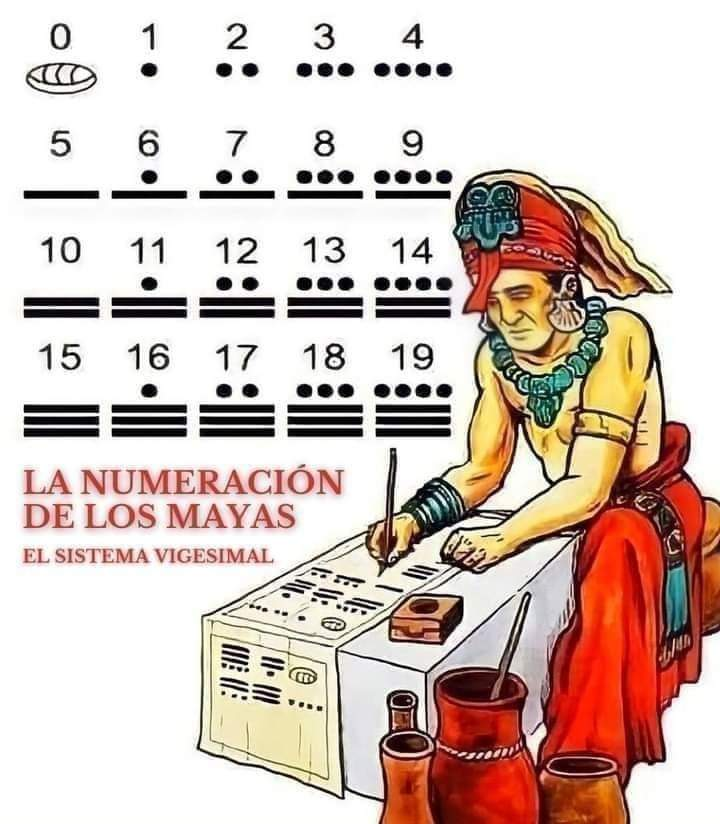
\includegraphics[width=0.5\textwidth,height=\textheight]{png/SistemaVigesimal.jpg}
\caption{\emph{Figura 1: El sistema vigesimal dels Maies}}
\end{figure}

\subsubsection{4.1.1 Sistemes de
numeració:}\label{sistemes-de-numeraciuxf3}

\begin{itemize}
\tightlist
\item
  \textbf{Binari (base 2):} Ús dels dígits 0 i 1.
\item
  \textbf{Octal (base 8):} Ús dels dígits del 0 al 7.
\item
  \textbf{Decimal (base 10):} Ús dels dígits del 0 al 9.
\item
  \textbf{Hexadecimal (base 16):} Ús dels dígits del 0 al 9 i les
  lletres A a F.
\end{itemize}

\emph{Taula 1: Exemples de codificació en diferents sistemes:}

\begin{longtable}[]{@{}rrrr@{}}
\toprule\noalign{}
Decimal & Binari & Octal & Hexadecimal \\
\midrule\noalign{}
\endhead
\bottomrule\noalign{}
\endlastfoot
0 & 0000 & 0 & 0 \\
1 & 0001 & 1 & 1 \\
2 & 0010 & 2 & 2 \\
3 & 0011 & 3 & 3 \\
4 & 0100 & 4 & 4 \\
5 & 0101 & 5 & 5 \\
6 & 0110 & 6 & 6 \\
7 & 0111 & 7 & 7 \\
8 & 1000 & 10 & 8 \\
9 & 1001 & 11 & 9 \\
10 & 1010 & 12 & A \\
15 & 1111 & 17 & F \\
16 & 10000 & 20 & 10 \\
17 & 10001 & 21 & 11 \\
31 & 11111 & 37 & 1F \\
\end{longtable}

\subsection{4.2 Exemples de conversió entre sistemes de
numeració.}\label{exemples-de-conversiuxf3-entre-sistemes-de-numeraciuxf3.}

A continuació es mostren alguns exemples de conversió entre sistemes de
numeració:

\subsubsection{1. Conversió de Binari a
Decimal}\label{conversiuxf3-de-binari-a-decimal}

\begin{itemize}
\item
  \textbf{Binari:} \texttt{1101}
\item
  \textbf{Decimal:}

  \(1 \times 2^3 + 1 \times 2^2 + 0 \times 2^1 + 1 \times 2^0\)

  \(= 8 + 4 + 0 + 1 = 13\)
\item
  \textbf{Decimal Resultat:} 13
\end{itemize}

\subsubsection{2. Conversió de Decimal a
Binari}\label{conversiuxf3-de-decimal-a-binari}

Exemple: 25,76

\paragraph{2.1 Part entera: 25}\label{part-entera-25}

\begin{itemize}
\item
  \textbf{Decimal:} 25
\item
  \textbf{Binari:}

  Dividim 25 per 2 i anotem els residus:

  \begin{itemize}
  \tightlist
  \item
    25 ÷ 2 = 12, residu = 1
  \item
    12 ÷ 2 = 6, residu = 0
  \item
    6 ÷ 2 = 3, residu = 0
  \item
    3 ÷ 2 = 1, residu = 1
  \item
    1 ÷ 2 = 0, residu = 1
  \end{itemize}

  Llegint els residus de baix a dalt: \texttt{11001}
\item
  \textbf{Binari Resultat:} 11001
\end{itemize}

\subsubsection{2.2 Part fraccionària ( decimal):
0,76}\label{part-fraccionuxe0ria-decimal-076}

0,76 × 2 = 1,52 → 1 (enter), 0,52 queda

0,52 × 2 = 1,04 → 1 (enter), 0,04 queda

0,04 × 2 = 0,08 → 0 (enter), 0,08 queda

0,08 × 2 = 0,16 → 0 (enter), 0,16 queda

0,16 × 2 = 0,32 → 0 (enter), 0,32 queda

0,32 × 2 = 0,64 → 0 (enter), 0,64 queda

0,64 × 2 = 1,28 → 1 (enter), 0,28 queda

0,28 × 2 = 0,56 → 0 (enter), 0,56 queda

0,56 × 2 = 1,12 → 1 (enter), 0,12 queda

Resultat aproximat: 0,76 en binari és \textbf{aproximadament}
0.110000101 (Pot no arribar a ser exacta.)

\subsubsection{3. Conversió de Hexadecimal a
Decimal}\label{conversiuxf3-de-hexadecimal-a-decimal}

\begin{itemize}
\item
  \textbf{Hexadecimal:} \texttt{1A3}
\item
  \textbf{Decimal:}

  Convertim cada dígit a decimal i utilitzem la base 16: (A = 10 en
  decimal)

  \begin{itemize}
  \tightlist
  \item
    \texttt{1A3} = \(1 \times 16^2 + A \times 16^1 + 3 \times 16^0\)
  \item
    \(= 1 \times 256 + 10 \times 16 + 3\)
  \item
    \(= 256 + 160 + 3 = 419\)
  \end{itemize}
\item
  \textbf{Decimal Resultat:} 419
\end{itemize}

\subsubsection{4. Conversió de Decimal a
Hexadecimal}\label{conversiuxf3-de-decimal-a-hexadecimal}

\begin{itemize}
\item
  \textbf{Decimal:} 255
\item
  \textbf{Hexadecimal:}

  Dividim 255 per 16 i anotem els residus:

  \begin{itemize}
  \tightlist
  \item
    255 ÷ 16 = 15, residu = 15
  \item
    15 en hexadecimal és \texttt{F}
  \end{itemize}

  Llegint els residus: \texttt{FF}
\item
  \textbf{Hexadecimal Resultat:} FF
\end{itemize}

\subsubsection{5. Conversió entre Hexadecimal i Binari (``automàtica''
de 1 a
4)}\label{conversiuxf3-entre-hexadecimal-i-binari-automuxe0tica-de-1-a-4}

\begin{itemize}
\item
  \textbf{Hexadecimal:} \texttt{A7}
\item
  \textbf{Binari:}

  Convertim cada dígit hexadecimal a binari (1 dígit H -\textgreater{} 4
  digits B)

  \begin{itemize}
  \tightlist
  \item
    A = 1010
  \item
    7 = 0111
  \end{itemize}

  Combina els resultats: \texttt{10100111}
\item
  \textbf{Binari Resultat:} 10100111
\end{itemize}

\subsubsection{6. Conversió entre Binari i Hexadecimal (``automàtica''
de 4 a
1)}\label{conversiuxf3-entre-binari-i-hexadecimal-automuxe0tica-de-4-a-1}

\begin{itemize}
\item
  \textbf{Binari:} \texttt{10101100}
\item
  \textbf{Hexadecimal:}

  Agrupem els bits en blocs de 4 (de dreta a esquerra):
  \texttt{1010\ 1100}

  \begin{itemize}
  \tightlist
  \item
    1010 = A
  \item
    1100 = C
  \end{itemize}

  Combina els resultats: \texttt{AC}
\item
  \textbf{Hexadecimal Resultat:} AC
\end{itemize}

Aquí tens exemples de conversió entre el sistema octal i el sistema
binari:

\subsubsection{7. Conversió de Octal a Binari (``Automàtica'' de 1 a
3)}\label{conversiuxf3-de-octal-a-binari-automuxe0tica-de-1-a-3}

\begin{itemize}
\item
  \textbf{Octal:} \texttt{345}

  Convertir cada dígit octal a binari (1 dígit O -\textgreater{} 3
  dígits B)

  \begin{itemize}
  \tightlist
  \item
    Octal \texttt{3} = Binari \texttt{011}
  \item
    Octal \texttt{4} = Binari \texttt{100}
  \item
    Octal \texttt{5} = Binari \texttt{101}
  \end{itemize}

  Combinar els resultats:

  \begin{itemize}
  \tightlist
  \item
    \texttt{345} en octal es converteix en \texttt{011\ 100\ 101} en
    binari.
  \end{itemize}
\end{itemize}

\subsubsection{8. Conversió de Binari a Octal (``Automàtica'' de 3 a
1)}\label{conversiuxf3-de-binari-a-octal-automuxe0tica-de-3-a-1}

\begin{itemize}
\item
  \textbf{Binari:} \texttt{100101011}

  Agrupar els dígits binaris en blocs de 3 (de dreta a esquerra):

  \begin{itemize}
  \tightlist
  \item
    \texttt{010\ 010\ 101\ 011}
  \end{itemize}

  Convertir cada grup de 3 dígits a octal:

  \begin{itemize}
  \tightlist
  \item
    Binari \texttt{010} = Octal \texttt{2}
  \item
    Binari \texttt{010} = Octal \texttt{2}
  \item
    Binari \texttt{101} = Octal \texttt{5}
  \item
    Binari \texttt{011} = Octal \texttt{3}
  \end{itemize}

  \textbf{Octal Resultat:} \texttt{2253}
\end{itemize}

\textbf{CONCLUSIONS:}

Les conversions entre octal i hexadecimal i binari són ``automàtiques''
perquè 8 i 16 són potències de 2 (8 = 2³; 16 = 2⁴).

\begin{itemize}
\tightlist
\item
  1 dígit octal \textless--\textgreater{} 3 dígits binaris
\item
  1 dígit hexadecimal \textless--\textgreater{} 4 dígits binaris
\end{itemize}

\emph{( A parir d'ací ho heu de llegir, no cal saber l'operativa)}

\subsection{4.3 Els enters: positius, zero(s) i
negatius.}\label{els-enters-positius-zeros-i-negatius.}

Hi ha diverses formes de representar els valors negatius. Les tres que
anem estudiar es caracteritzen per destinar el MSB ( Bit major, el de la
dreta) a indicar el signe:

\begin{itemize}
\item
  1: Negatiu
\item
  0: Positiu
\end{itemize}

Això implica que ``perdem'' un bit per representar valors.

\subsubsection{4.3.1 Bit amb signe}\label{bit-amb-signe}

Es reserva el primer bit per indicar el signe

\begin{itemize}
\item
  \textbf{0}0000011 -\textgreater{} 3
\item
  \textbf{1}0000011 -\textgreater{} -3
\end{itemize}

\subsubsection{4.3.2 Complement a 1}\label{complement-a-1}

Els negatius es codifiquen fent l'inversa de cada bit. No té ús, el
veiem per entendre el Complement a 2.

\emph{Taula 2: Exemples d'enters en Ca1}

\begin{longtable}[]{@{}lr@{}}
\toprule\noalign{}
Byte en complement a 1 & Decimal \\
\midrule\noalign{}
\endhead
\bottomrule\noalign{}
\endlastfoot
00000000 & (positiu) 0 \\
11111111 & (negatiu) 0 \\
00000001 & 1 \\
00000010 & 2 \\
00000011 & 3 \\
00000100 & 4 \\
11111110 & -1 \\
11111101 & -2 \\
11111100 & -3 \\
11111011 & -4 \\
\end{longtable}

\textbf{Rang i combinacions en Ca1:}

En 1 byte pot representar 2⁸=256 combinacions diferents. Rang de valors
representables: Nombres positius: 0 a 2⁷−1=127 (el bit més significatiu
és 0). Nombres negatius: −1 a −2⁷+1=−127 (el bit més significatiu és 1).
En complement a 1, tenim dos zeros (0 positiu: 00000000 i 0 negatiu:
11111111).

Així doncs, el rang de valors és de -127 a 127, incloent els dos zeros.
Per tant, encara que tinguem 256 combinacions, representem 255 números
diferents (perquè dos d'ells són el mateix nombre 0).

\subsubsection{4.3.3 Complement a 2}\label{complement-a-2}

Per solucionar el problema dels 2 zeros i aprofitar millor totes les
representacions, el que fem en els negatius és restar un 1 al Ca1. Ca1
de -1 -\textgreater{} 0000 0001 -\textgreater{} 1111 1110

Ca1 de -7 -\textgreater{} 0000 0111 -\textgreater{} 1111 1000

Ca1 de 0 -\textgreater{} 0000 0000 -\textgreater{} 1111

Ca1 de -1 -\textgreater{} 0000 0001 -\textgreater{} 1111 1110 +1
-\textgreater{} 1111 1111

Ca2 de -7 -\textgreater{} 0000 0111 -\textgreater{} 1111 1000 +1
-\textgreater{} 1111 1010

Ca2 de 0 -\textgreater{} 0000 0000 -\textgreater{} 1111 1111
-\textgreater{} 0000 0000 (overflow)

\emph{Taula 3: Exemples d'enters en Ca2}

\begin{longtable}[]{@{}lr@{}}
\toprule\noalign{}
Byte en complement a 2 & Decimal \\
\midrule\noalign{}
\endhead
\bottomrule\noalign{}
\endlastfoot
00000000 & 0 \\
00000001 & 1 \\
00000010 & 2 \\
00000011 & 3 \\
00000100 & 4 \\
11111111 & -1 \\
11111110 & -2 \\
11111101 & -3 \\
11111100 & -4 \\
\end{longtable}

Per obtenir el valor en decimal:

Si MSB ( bit major) = 1; Restem un 1 i després invertim:

1111 1101 -\textgreater{} 1111 1100 -\textgreater{} 0000 0011
-\textgreater{} -3

\textbf{Rang i combinacions en Ca2:}

En 1 byte pot representar 2⁸=256 combinacions diferents. Rang de valors
representables: Nombres positius: 0 a 2⁷−1=127 (el bit més significatiu
és 0). Nombres negatius: −1 a −2⁷=−128 (el bit més significatiu és 1).
En complement a 2, sols tenim un 0

Així doncs, el rang de valors és de -128 a 127. Per tant, les 256
combinacions, representem 256 números diferents-

\subsection{4.4 Els números reals}\label{els-nuxfameros-reals}

Exemples de números reals: * 3,141592653589793 * 3 * -3 * 0 *
34.354.656.757.885.334.343 * 0,000000000000000000000000000000000103

Per tant: els reals inclouen als números enters (-2 = -2,000; 34 =
34,000) que inclouen als naturals.

\subsubsection{4.4.1 Coma flotant.
General.}\label{coma-flotant.-general.}

Els formats en FP ens permeten guardar qualsevol número siga quin siga
el seu pes (alt o baix)

\textbf{Parts:}

\begin{itemize}
\tightlist
\item
  Mantissa: Conté un valor del tipus 0,1XXXX
\item
  Exponent: Per a fer el valor
\end{itemize}

\textbf{Procés:}

1- Normalització de la mantissa: S'ajusta el valor al primer \textbf{bit
significatiu}: 0,\emph{1}xxxxx 2- Bit implícit. Omitim el 1r bit. 3- Es
calcula l'exponent i se li suma a l'excés. Amb l'excés fem que els
exponents siguen sempre psoitius i no ``perdem'' el MSB per a indicar el
signe.

\subsubsection{4.4.2 Estàndards}\label{estuxe0ndards}

Els dos formats estàndard de coma flotant segons l'estàndard IEEE 754
són:

\begin{enumerate}
\def\labelenumi{\arabic{enumi}.}
\tightlist
\item
  \textbf{Simple precisió (32 bits)}:

  \begin{itemize}
  \tightlist
  \item
    \textbf{1 bit} per al signe.
  \item
    \textbf{8 bits} per a l'exponent, amb biaix de 127.
  \item
    \textbf{23 bits} per a la mantissa (fracció). Un bit addicional,
    implícit, sempre és 1 i no s'emmagatzema (mantissa normalitzada).
  \item
    \textbf{Rang:} Aproximadament de \(-3.4 \times 10^{38}\) a
    \(3.4 \times 10^{38}\).
  \end{itemize}
\item
  \textbf{Doble precisió (64 bits)}:

  \begin{itemize}
  \tightlist
  \item
    \textbf{1 bit} per al signe.
  \item
    \textbf{11 bits} per a l'exponent, amb biaix de 1023.
  \item
    \textbf{52 bits} per a la mantissa. Igual que en simple precisió, té
    un bit implícit.
  \item
    \textbf{Rang:} Aproximadament de \(-1.8 \times 10^{308}\) a
    \(1.8 \times 10^{308}\).
  \end{itemize}
\end{enumerate}

Aquests formats permeten representar nombres molt grans o molt petits
amb precisió controlada.Independentment de que representen un nombre amb
part fraccionària o un enter.

\emph{(A partir d'ací cal estudiar)}

\section{5 Sobre els usos habituals de cada sistema de
numeració}\label{sobre-els-usos-habituals-de-cada-sistema-de-numeraciuxf3}

\begin{enumerate}
\def\labelenumi{\arabic{enumi}.}
\item
  El BINARI és com es codifica la informació al SI internament. El
  hardware només usa 0/1.
\item
  Al món humà usem el DECIMAL (0-9) o SEXAGESIMAL (0-59) (minuts, segons
  o graus dels angles).
\item
  Els perifèrics d'entrada i eixida tradueixen o codifiquen informació
  del món humà: * assignant-li valors numèrics a cada color, X,Y,
  intensitat de so, dia-hores-minuts-segon\ldots{} o * llegint
  directament el valor que introduim d'imports, kilos, metres\ldots{}
\end{enumerate}

De decimal o sexagesimal a binari (entrada) o a la inversa (eixida)

\begin{enumerate}
\def\labelenumi{\arabic{enumi}.}
\setcounter{enumi}{3}
\tightlist
\item
  L'OCTAL (0-7), HEXAGESIMAL (0-9,A-F) i el DECIMAL és usat pel software
  de les interfícies per \textbf{facilitar-nos} la lectura de dades
  com,per exemple, adreces IP, adreces MAC, colors, permisos de fitxers
  en Linux, adreces de memòria\ldots{} Llegir i recordar valors en
  binari és complicadíssim i es presta a errors.
\end{enumerate}

\subsection{5.1 Exemple de la codificació del color
RGB.}\label{exemple-de-la-codificaciuxf3-del-color-rgb.}

El codi de color es guarda internament en 3 bytes o siga 24 bits però el
software pot mostrar/admetre:

\begin{itemize}
\tightlist
\item
  3 decimals que val cadascuna del 0 al 255.
\item
  1 hexadecimal que val cadascun de 000000 a FFFFFF. Ací observem la
  comodidat del Hexadecimal
\end{itemize}

\emph{Taula 4: Exemples de RGB en hexadecimal, decimals i el binari}

\begin{longtable}[]{@{}
  >{\raggedright\arraybackslash}p{(\columnwidth - 6\tabcolsep) * \real{0.1194}}
  >{\raggedright\arraybackslash}p{(\columnwidth - 6\tabcolsep) * \real{0.1791}}
  >{\raggedright\arraybackslash}p{(\columnwidth - 6\tabcolsep) * \real{0.2388}}
  >{\raggedright\arraybackslash}p{(\columnwidth - 6\tabcolsep) * \real{0.4627}}@{}}
\toprule\noalign{}
\begin{minipage}[b]{\linewidth}\raggedright
Color
\end{minipage} & \begin{minipage}[b]{\linewidth}\raggedright
Hexadecimal
\end{minipage} & \begin{minipage}[b]{\linewidth}\raggedright
RGB (Decimal)
\end{minipage} & \begin{minipage}[b]{\linewidth}\raggedright
RGB (Binari)
\end{minipage} \\
\midrule\noalign{}
\endhead
\bottomrule\noalign{}
\endlastfoot
Negre & \#000000 & (0, 0, 0) & (00000000, 00000000, 00000000) \\
Blanc & \#FFFFFF & (255, 255, 255) & (11111111, 11111111, 11111111) \\
Roig & \#FF0000 & (255, 0, 0) & (11111111, 00000000, 00000000) \\
Verd & \#00FF00 & (0, 255, 0) & (00000000, 11111111, 00000000) \\
Blau & \#0000FF & (0, 0, 255) & (00000000, 00000000, 11111111) \\
Taronja & \#FF8242 & (255,130,65) & (11111111, 10000010, 01000001) \\
\end{longtable}

Quan introduim o llegim el valor no fem ús del binari però és com es
guarda.

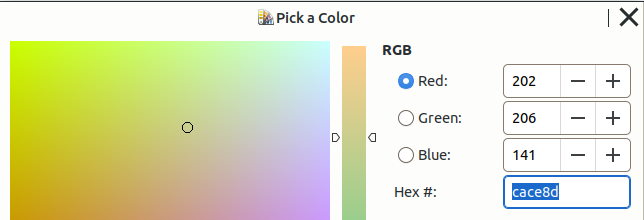
\includegraphics{png/RGB.png}

\begin{quote}
\textbf{Resumint:}

1- La màquina NOMÉS treballa en BINARI

2- El decimal, l'octal i l'hexadecimal, són «traduccions» que ens
ofereixen les interfície software per a facilitar la lectura i
escriptura d'aquests valors als humans.

És és fácil llegir a la pantalla i introduir pel teclat: CACE8D que el
valor que realment es guarda memòria o CPU: 110010101100111010001101
\end{quote}

\section{6. Els caràcters. La representació dels
alfanumèrics}\label{els-caruxe0cters.-la-representaciuxf3-dels-alfanumuxe8rics}

Tipus:

\begin{itemize}
\item
  Alfanumèrics: 0-9, a-z, A-Z
\item
  Amb tilles ö, ü., à
\item
  Especials: \^{} ! ``\,'' ?\ldots{}
\item
  De control (no visibles): LF, CR\ldots{}
\end{itemize}

\subsection{6.1 Evolució: de l'ASCII al
UTF}\label{evoluciuxf3-de-lascii-al-utf}

Inicialment els caràcter es van codificar en ASCII (American Standard
Code for Information Interchange). Utilitza 7 o 8 bits. (En origen, 7 en
anglés)

\begin{itemize}
\item
  \textbf{ASCII} estava limitat a 128 caràcters en l'original anglès.
  Limitat a 256 en la versió extesa de 8 bits posterior, la qual cosa no
  era suficient per representar tots els caràcters necessaris per a
  diferents idiomes com el xinès, japonès o àrab.
\item
  \textbf{Pàgines de codi} Donades estes limitacions d'ASCII es van anar
  creant conjunts (set char) específics de caràcters per a diferents
  grups d'idiomes o regions. Per exemple ISO 8859-1 per a l'Europa
  Occidental (Latin-1) o la ISO 8859-5 per al ciríl·lic. Però apareixien
  els problemes de compatibilitat entre pàgines web i fitxers.
\item
  \textbf{Unicode} va ser dissenyat per superar aquestes limitacions,
  permetent la representació de caràcters de pràcticament tots els
  sistemes d'escriptura coneguts. UTF-8, un dels formats de codificació
  de Unicode, és compatible amb ASCII però permet la codificació de
  caràcters addicionals utilitzant múltiples bytes.
\end{itemize}

\subsection{6.2 Codificacions UTF}\label{codificacions-utf}

\emph{(Només llegir)}

Les codificacions UTF (Unicode Transformation Format) més comuns són
UTF-8, UTF-16 i UTF-32.

\subsubsection{UTF-8 (Unicode Transformation Format de 8
bits)}\label{utf-8-unicode-transformation-format-de-8-bits}

\begin{itemize}
\tightlist
\item
  \textbf{Mida del Codi}: Variable, de 1 a 4 bytes.
\item
  \textbf{Compatibilitat}: Compatible amb ASCII per als primers 128
  caràcters.
\item
  \textbf{Ús}: És el format de codificació més utilitzat a la web i en
  molts sistemes moderns. És eficient en espai per a textos que
  utilitzen principalment caràcters ASCII.
\end{itemize}

\subsubsection{UTF-16 (Unicode Transformation Format de 16
bits)}\label{utf-16-unicode-transformation-format-de-16-bits}

\begin{itemize}
\tightlist
\item
  \textbf{Mida del Codi}: Variable, de 2 a 4 bytes.
\item
  \textbf{Compatibilitat}: Pot utilitzar una seqüència de 2 bytes o 4
  bytes.
\item
  \textbf{Ús}: Comú en sistemes com Windows i moltes aplicacions de
  programació. És més eficient per a textos amb molts caràcters no
  ASCII.
\end{itemize}

\subsubsection{UTF-32 (Unicode Transformation Format de 32
bits)}\label{utf-32-unicode-transformation-format-de-32-bits}

\begin{itemize}
\tightlist
\item
  \textbf{Mida del Codi}: Fix, 4 bytes per a cada caràcter.
\item
  \textbf{Compatibilitat}: Representa directament cada caràcter Unicode
  en un sol valor de 32 bits.
\item
  \textbf{Ús}: Menys eficient en termes d'espai en comparació amb UTF-8
  i UTF-16, però simplifica la manipulació de caràcters perquè cada
  caràcter té una longitud fixa.
\end{itemize}

Hi ha altres Codificacions UTF

\subsection{6.3 UTF-8 i Latin-1}\label{utf-8-i-latin-1}

La diferència principal entre \textbf{UTF-8} i \textbf{Latin1} (també
conegut com a \textbf{ISO-8859-1}) rau en com codifiquen els caràcters i
la quantitat de caràcters que poden representar. * UTF-8 és una
codificació de longitud variable: un caràcter pot ocupar entre 1 i 4
bytes. És la codificació més actual i pot codificar una àmplia gamma de
caràcters sent compatible amb els anteriors ASCII.

\begin{itemize}
\tightlist
\item
  Latin1 és una codificació d'un sol byte, té una cobertura limitada en
  només poder representar fins a 256 caràcters (de 0 a 255): els
  caràcters bàsics d'anglès i diversos caràcters accentuats de llengües
  europees occidentals, però no pot representar caràcters d'altres
  idiomes, com el xinès o l'àrab, ni molts símbols especials.
\end{itemize}

Els primers 128 caràcters en UTF-8 són idèntics als d'ASCII original de
7 bits (anglés) i la resta de pàgines.

\emph{Taula 5: Exemples de caràctersn en diferents codificacions}

\begin{longtable}[]{@{}
  >{\raggedright\arraybackslash}p{(\columnwidth - 8\tabcolsep) * \real{0.1316}}
  >{\raggedright\arraybackslash}p{(\columnwidth - 8\tabcolsep) * \real{0.1842}}
  >{\raggedright\arraybackslash}p{(\columnwidth - 8\tabcolsep) * \real{0.2368}}
  >{\raggedright\arraybackslash}p{(\columnwidth - 8\tabcolsep) * \real{0.1974}}
  >{\raggedright\arraybackslash}p{(\columnwidth - 8\tabcolsep) * \real{0.2500}}@{}}
\toprule\noalign{}
\begin{minipage}[b]{\linewidth}\raggedright
Caràcter
\end{minipage} & \begin{minipage}[b]{\linewidth}\raggedright
UTF-8 (Hex)
\end{minipage} & \begin{minipage}[b]{\linewidth}\raggedright
UTF-8 (Decimal)
\end{minipage} & \begin{minipage}[b]{\linewidth}\raggedright
Latin-1 (Hex)
\end{minipage} & \begin{minipage}[b]{\linewidth}\raggedright
Latin-1 (Decimal)
\end{minipage} \\
\midrule\noalign{}
\endhead
\bottomrule\noalign{}
\endlastfoot
\textbf{à} & \texttt{C3\ A0} & \texttt{195\ 160} & \texttt{E0} &
\texttt{224} \\
\textbf{ñ} & \texttt{C3\ B1} & \texttt{195\ 177} & \texttt{F1} &
\texttt{241} \\
\textbf{ç} & \texttt{C3\ A7} & \texttt{195\ 167} & \texttt{E7} &
\texttt{231} \\
\emph{a} & \texttt{61} & \texttt{97} & \texttt{61} & \texttt{97} \\
\emph{7} & \texttt{37} & \texttt{55} & \texttt{37} & \texttt{55} \\
\emph{-} & \texttt{2D} & \texttt{45} & \texttt{2D} & \texttt{45} \\
\emph{'} & \texttt{27} & \texttt{39} & \texttt{27} & \texttt{39} \\
\end{longtable}

\subsubsection{Resum:}\label{resum}

\begin{itemize}
\tightlist
\item
  \textbf{UTF-8}: Més flexible i versàtil, amb suport per a quasi tots
  els caràcters possibles.
\item
  \textbf{Latin1}: Més senzill i lleuger, però amb una cobertura de
  caràcters molt limitada, adequada només per a llengües europees
  occidentals.
\end{itemize}

\subsection{6.3 Activitat proposta. Compatibilitat i conversió entre
pàgines de codi i
UTF-8.}\label{activitat-proposta.-compatibilitat-i-conversiuxf3-entre-puxe0gines-de-codi-i-utf-8.}

Descarreguem un fitxer de dades de tipus CSV (Comma Separated Values)
del INE (Instituto Nacional de Estadística) i, en intentar obrir-lo,
observem que apareixen uns caràcters estranys (com errors).

\emph{Què està passant?}

El Libreoffice està interpretant-lo amb com si haguera estat codificat
en \textbf{UTF-8}:

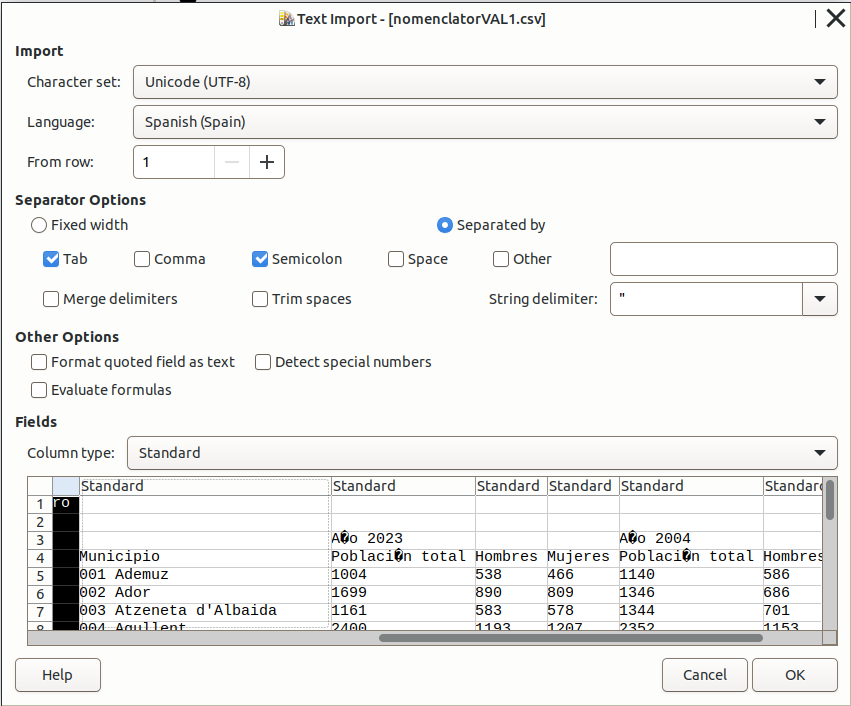
\includegraphics[width=0.75\textwidth,height=\textheight]{png/csv1.png}

\emph{Com ho solucionem?}

Com intuim que l'idioma deu ser un idioma europeu, provem canviant el
conjunt de caràcters a \textbf{Latin-1} que deu ser el conjunt usat en
la codificació:

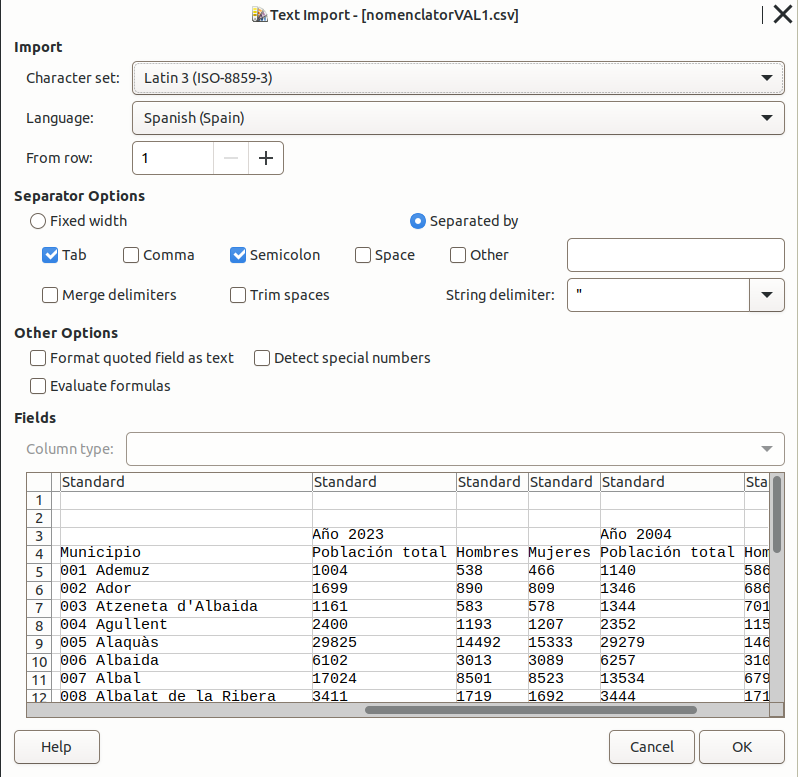
\includegraphics[width=0.75\textwidth,height=\textheight]{png/csv2.png}

\emph{Seguim investigant}

Preguntem a ChatGPT per alguna eina per convertir textos (o fitxers de
text) d'un conjunt de caràcters a un altre. Ens proposa l'ordre de Linux
``iconv''.

\emph{Convertim el fitxer de Latin-1 a UTF8}

Usem l'ordre amb l'ajuda de ChatGPT per converti un fitxer (-f) de text
pla com són els CSV que venia codificat en Latin-1 a UTF8

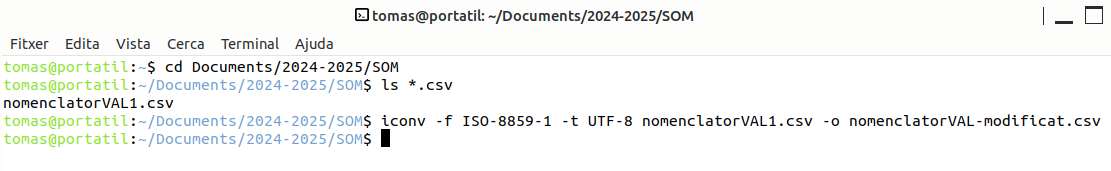
\includegraphics[width=0.75\textwidth,height=\textheight]{png/iconv.png}

Comprovem que ara sí es pot obrir com fitxer codificat en UTF8

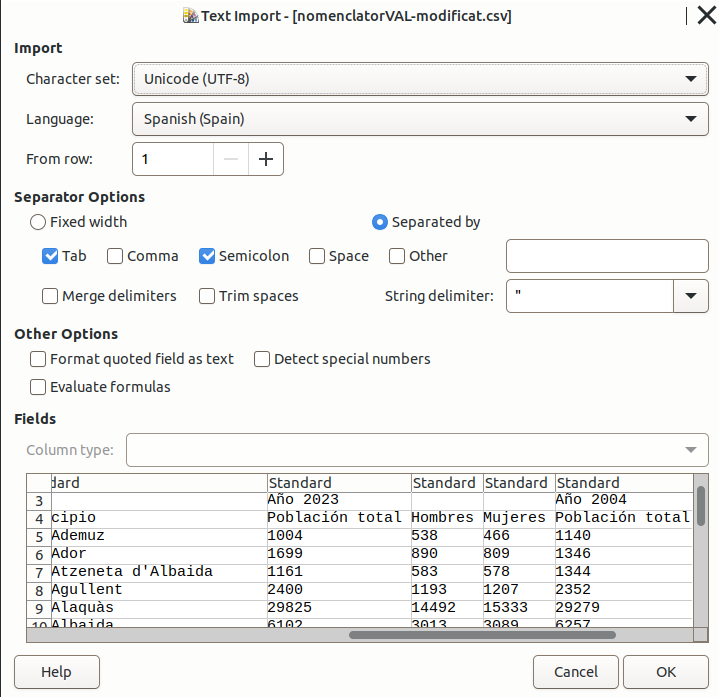
\includegraphics[width=0.75\textwidth,height=\textheight]{png/csv3.png}

\emph{Presta més atenció, sigues curiós\ldots{}}

Com a detall, si observem el tamany dels fitxers, aquest es un poc
diferent.

\begin{itemize}
\tightlist
\item
  El fitxer codificat en Latin-1 mesura 8250 bytes
\item
  El fitxer recodificat a UTF8 mesura 8420 bytes.
\end{itemize}

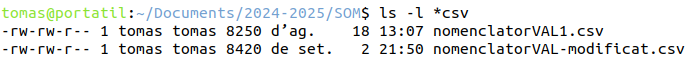
\includegraphics{png/ls.png}

També ho podem vore des del GUI

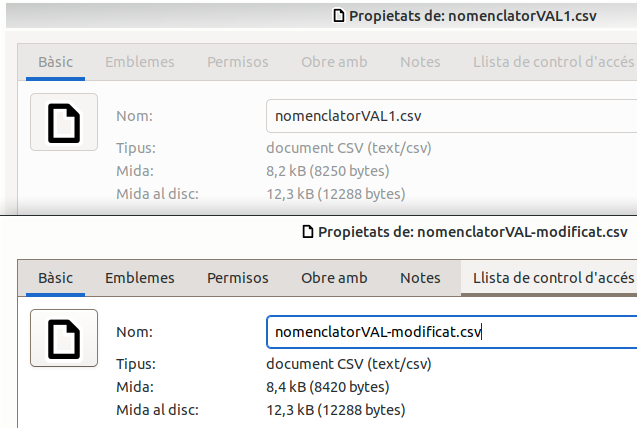
\includegraphics{png/ls2.png}

\textbf{A què creus que pot deure's?}

\section{7. Els diferents tipus en els
llenguatges}\label{els-diferents-tipus-en-els-llenguatges}

\emph{(Només llegir)}

Quan usem un llenguatge de programació (Python, R, C, Java, Javascript,
PHP) o també un llenguatge d'scripts, definirem variables on guardarem
temporalment valors numèrics, alfanumèrics o booleanes tal com les hem
estudiades.

\begin{itemize}
\tightlist
\item
  El següent codi correspon a un fitxer de C
\item
  Crea variables de diferents tipus,
\item
  Els assigna valors,
\item
  Imprimeix el seu tamanay \emph{(sizeof())}
\end{itemize}

\begin{Shaded}
\begin{Highlighting}[]
\PreprocessorTok{\#include }\ImportTok{\textless{}stdio.h\textgreater{}}

\DataTypeTok{int}\NormalTok{ main}\OperatorTok{()} \OperatorTok{\{}
    \CommentTok{// Tipus numèrics en C}
    \DataTypeTok{char}\NormalTok{ c }\OperatorTok{=} \CharTok{\textquotesingle{}A\textquotesingle{}}\OperatorTok{;}                    \CommentTok{// Enter de 8 bits (1 byte)}
    \DataTypeTok{short}\NormalTok{ s }\OperatorTok{=} \DecValTok{32767}\OperatorTok{;}                 \CommentTok{// Enter curt de 16 bits (2 bytes)}
    \DataTypeTok{int}\NormalTok{ i }\OperatorTok{=} \DecValTok{2147483647}\OperatorTok{;}              \CommentTok{// Enter de 32 bits (4 bytes)}
    \DataTypeTok{long}\NormalTok{ l }\OperatorTok{=} \DecValTok{9223372036854775807}\BuiltInTok{L}\OperatorTok{;}   \CommentTok{// Enter llarg de 64 bits (8 bytes)}
    \DataTypeTok{long} \DataTypeTok{long}\NormalTok{ ll }\OperatorTok{=} \DecValTok{9223372036854775807}\BuiltInTok{LL}\OperatorTok{;} \CommentTok{// Enter molt llarg de 64 bits (8 bytes)}
    \DataTypeTok{float}\NormalTok{ f }\OperatorTok{=} \FloatTok{3.14}\BuiltInTok{f}\OperatorTok{;}                 \CommentTok{// Punt flotant de precisió simple (4 bytes)}
    \DataTypeTok{double}\NormalTok{ d }\OperatorTok{=} \FloatTok{3.141592653589793}\OperatorTok{;}    \CommentTok{// Punt flotant de doble precisió (8 bytes)}
    \DataTypeTok{long} \DataTypeTok{double}\NormalTok{ ld }\OperatorTok{=} \FloatTok{3.141592653589793238}\BuiltInTok{L}\OperatorTok{;} \CommentTok{// Punt flotant de precisió estesa (12{-}16 bytes, depèn del sistema)}

    \CommentTok{// Mostrar el tamany de cada tipus}
\NormalTok{    printf}\OperatorTok{(}\StringTok{"Tamany de char: }\SpecialCharTok{\%zu}\StringTok{ bytes}\SpecialCharTok{\textbackslash{}n}\StringTok{"}\OperatorTok{,} \KeywordTok{sizeof}\OperatorTok{(}\NormalTok{c}\OperatorTok{));}
\NormalTok{    printf}\OperatorTok{(}\StringTok{"Tamany de short: }\SpecialCharTok{\%zu}\StringTok{ bytes}\SpecialCharTok{\textbackslash{}n}\StringTok{"}\OperatorTok{,} \KeywordTok{sizeof}\OperatorTok{(}\NormalTok{s}\OperatorTok{));}
\NormalTok{    printf}\OperatorTok{(}\StringTok{"Tamany de int: }\SpecialCharTok{\%zu}\StringTok{ bytes}\SpecialCharTok{\textbackslash{}n}\StringTok{"}\OperatorTok{,} \KeywordTok{sizeof}\OperatorTok{(}\NormalTok{i}\OperatorTok{));}
\NormalTok{    printf}\OperatorTok{(}\StringTok{"Tamany de long: }\SpecialCharTok{\%zu}\StringTok{ bytes}\SpecialCharTok{\textbackslash{}n}\StringTok{"}\OperatorTok{,} \KeywordTok{sizeof}\OperatorTok{(}\NormalTok{l}\OperatorTok{));}
\NormalTok{    printf}\OperatorTok{(}\StringTok{"Tamany de long long: }\SpecialCharTok{\%zu}\StringTok{ bytes}\SpecialCharTok{\textbackslash{}n}\StringTok{"}\OperatorTok{,} \KeywordTok{sizeof}\OperatorTok{(}\NormalTok{ll}\OperatorTok{));}
\NormalTok{    printf}\OperatorTok{(}\StringTok{"Tamany de float: }\SpecialCharTok{\%zu}\StringTok{ bytes}\SpecialCharTok{\textbackslash{}n}\StringTok{"}\OperatorTok{,} \KeywordTok{sizeof}\OperatorTok{(}\NormalTok{f}\OperatorTok{));}
\NormalTok{    printf}\OperatorTok{(}\StringTok{"Tamany de double: }\SpecialCharTok{\%zu}\StringTok{ bytes}\SpecialCharTok{\textbackslash{}n}\StringTok{"}\OperatorTok{,} \KeywordTok{sizeof}\OperatorTok{(}\NormalTok{d}\OperatorTok{));}
\NormalTok{    printf}\OperatorTok{(}\StringTok{"Tamany de long double: }\SpecialCharTok{\%zu}\StringTok{ bytes}\SpecialCharTok{\textbackslash{}n}\StringTok{"}\OperatorTok{,} \KeywordTok{sizeof}\OperatorTok{(}\NormalTok{ld}\OperatorTok{));}

    \ControlFlowTok{return} \DecValTok{0}\OperatorTok{;}
\OperatorTok{\}}
\end{Highlighting}
\end{Shaded}

El resultat, després de compilar i executar el programa .exe resultant
serà:

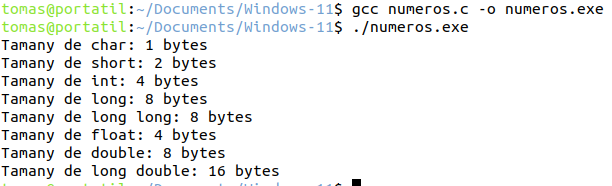
\includegraphics[width=0.5\textwidth,height=\textheight]{png/numeros.exe.png}

\section{8. Dades complexes. La gràfica de la
informació}\label{dades-complexes.-la-gruxe0fica-de-la-informaciuxf3}

Hem vist la codificació de dades simples (caràcters alfanumèrics, de
control, valors numèrics\ldots) i les possibles formes de codificar-les.

Ara hem d'entendre que un import, un descompte, una edat, un color, el
sexe, Vacunat contra el COVID?\ldots pot representar-se com a nombre o
lletra. El llegirem en decimal, hexadecimal, caràcter\ldots{} però es
gravarà en binari (Ca2, Bit Sense Signe, hexadecimal, M/F, TRUE/FALSE).

Es tracta de dades simples. Les dades complexes que es tracten en altres
temes (fitxers, Bases de dades, llenguatges de marques\ldots{} ) són
composicions o combinacions estructurades d'aquestes dades simples:

\begin{itemize}
\tightlist
\item
  \textbf{Píxels:} Elements mínims d'una imatge digital. Es defineixen
  per una coordenada X i un Y (dos números) -\textbf{Resolució:} Nombre
  de píxels en una imatge (ex. 1920x1080).
\item
  \textbf{Profunditat de color:} Nombre de bits per píxel (ex. 24 bits
  per color RGB).
\end{itemize}

\section{7. Més sobre la
codificació}\label{muxe9s-sobre-la-codificaciuxf3}

Fins el moment hem parat de la informació estricta, és a dir, allò que
té un significat. El preu, el color, els anys, el \% de malalts, el
volumen\ldots{}

Però en guardar la informació -o en enviar-la- els nostres sistemes
solen fer dos procesos previs que modifiquen la codificació esperada del
binari. Es tracta de dos procesos que afecten al tamany esperat de forma
distinta:

\begin{itemize}
\item
  Afegir bits per al tractamet de possibles errors.
\item
  Comprimir: recodificar el binari per reduir l'espai físic (bits
  totals) que ocupa.
\end{itemize}

\subsection{7.1 Detecció o correcció
d'errors}\label{detecciuxf3-o-correcciuxf3-derrors}

( Es tracta d'uns bits addicionals (no aporten informació) que s'afigen
a tot el bloc d'informació (o a cada byte) per a detectar i alguns per
corregir si hi s'ha produït un error en l'enviament a través de les
xarxes o magatzematge.

\begin{itemize}
\item
  \textbf{Bits de paritat:} Afegir un bit addicional per fer que el
  nombre de 1 (o de 0) siga parell.
\item
  \textbf{CRC (Cyclic Redundancy Check):} Genera un valor de verificació
  que es compara per assegurar la integritat de les dades.
\item
  \textbf{Checksum:} Similar al CRC, suma tots els bytes d'un conjunt de
  dades per produir un valor que es compara per detectar errors simples.
\item
  \textbf{Hash (Funcions de hash):} Crea un codi únic per a un conjunt
  de dades. És útil per a la integritat de fitxers, autenticació i
  emmagatzematge segur de contrasenyes, però no està pensat per a la
  correcció d'errors. L'usarem més avant quan descarreguem paquets de
  software grans com la ISO de Lubuntu, Windows 11\ldots{} En la Unitat
  2 provarem una funció Hash.
\item
  \textbf{ECC (Error-Correcting Code):} Utilitzat en memòries RAM per
  corregir errors simples o dobles en dades, millorant la fiabilitat del
  sistema.
\item
  \textbf{Hamming Code:} Codi de correcció que pot detectar i corregir
  errors simples d'un sol bit en la transmissió de dades. \#\# 7.2
  Compressió de dades
\end{itemize}

\emph{(Només cal llegir. Tractarem la compressió més avant)}

Es basen en dos tècniques.

\begin{itemize}
\item
  \textbf{Huffman:} Mètode de compressió sense pèrdua que utilitza codis
  de longitud variable. Destina cadenes de bits més curtes per a
  codificar els valors més freqüents. L'usa el JPEG i el MP3.
\item
  \textbf{Run-Length Encoding (RLE):} Compressió que representa
  seqüències repetides d'un valor amb una sola instància i la seua
  quantitat. Molt potent quan les dades es repeteixen molt. L'usa el
  format BMP (algunes versions) i TIFF.
\end{itemize}

En el cas de les imatges ja existeixen formats de fitxers comprimits:

\begin{itemize}
\tightlist
\item
  \textbf{BMP:} Format sense compressió (estàndard tradicional)
\item
  \textbf{JPEG:} Format amb compressió amb pèrdua.
\item
  \textbf{PNG:} Format amb compressió sense pèrdua.
\end{itemize}

\end{document}
